\documentclass[12pt,a4paper]{article}

\usepackage{fontspec}
\defaultfontfeatures{Ligatures=TeX}
\setmainfont[
  Path={fonts/TH Sarabun PSK V-1/},
  Extension=.ttf,
  UprightFont={*},
  BoldFont={* Bold},
  ItalicFont={* Italic},
  BoldItalicFont={* BoldItalic}
]{THSarabun}
\setmonofont{Latin Modern Mono}

\usepackage{graphicx}
\usepackage{textcomp}
\usepackage{amsmath,amssymb,float,caption,subcaption,xcolor,hyperref,fancyhdr,tikz}
\usetikzlibrary{positioning,arrows.meta,calc}
\usepackage{geometry,booktabs,array,tabularx}
\geometry{margin=1in}
\setlength{\headheight}{14.5pt}
\pagestyle{fancy}\fancyhf{}\lhead{IBR Grid-Following / Grid-Forming: State Order and Small-Signal Stability}\rhead{\thepage}
\hypersetup{colorlinks=true,linkcolor=blue,urlcolor=blue,citecolor=blue}
\renewcommand{\arraystretch}{1.12}
\captionsetup[table]{skip=7pt}
\emergencystretch=2em
\linespread{1.12}

\title{\textbf{Reduced 6-state Inverter-Based Resource (IBR) Models: Grid-Following and Grid-Forming}\\
\large State Order, Small-Signal Stability (SSSA), and $i_d/i_q/P/Q$ Comparison on a SMIB}
\date{22 July 2026}

\begin{document}
\maketitle

\begin{abstract}
This report documents the \emph{state order} of two reduced-order IBR models,
\textbf{6 states each}, implemented as project-owned MATLAB code following the
EECON49 formulation and connected to an ideal infinite bus through $Z_{line}$
(single-machine infinite-bus, SMIB): (i) a \textbf{Grid-Following (GFL) 6-state}
model and (ii) a \textbf{Grid-Forming VSG (GFM) 6-state} model. Each is organised
into \emph{three blocks of two states}: GFL = IBR + GFL(PLL) + PQ, and GFM = IBR +
VSG + GFM. The report presents only the \textbf{Small-Signal Stability (SSSA)}
results (eigenvalue spectrum with a complex-plane plot and a modal-frequency (Hz)
chart) and the $i_d,i_q,P,Q$ equilibrium and time-domain ring-down; power-flow
results are deliberately omitted. Both models exhibit the physically expected
\emph{oscillatory (complex) mode}: a PLL mode near $0.34$ Hz for the GFL and a
swing mode near $10.8$ Hz for the GFM. All equations are traceable to cited
sources; no parameter was tuned to match any target.
\end{abstract}
\newpage
\tableofcontents
\newpage

\section{Scope and Source Discipline}

This report focuses on the state structure and SSSA results of the reduced 6-state
IBR models; power-flow verification is out of scope (per the user's request to omit
PF). The structure and numeric values follow the EECON49-P4 formulation~\cite{eecon49};
the block-level equations trace to standard references:

\begin{itemize}
  \item \textbf{GFL 6-state.} The current control and SRF-PLL are
  \texttt{SOURCE\_DEFINED} from Yazdani \& Iravani~\cite{yazdani2010} and
  Teodorescu et al.~\cite{teodorescu2011}; the outer PQ power loop is
  \texttt{APPROVED\_PROJECT\_DERIVED} following Bacha et al.~\cite{bacha2014}.
  \item \textbf{GFM 6-state.} The virtual swing (VSG) and Q-V droop voltage forming
  trace to the VSG literature (Pogaku et al.~\cite{pogaku2007}, Sakimoto et
  al.~\cite{sakimoto2015}); the 6-state reduced assembly is
  \texttt{PROJECT\_DERIVED\_SOURCE\_MAPPED}.
\end{itemize}

The reduction to 6 states removes the power/voltage measurement filters and the
current-loop integrators (leaving proportional + decoupling current control), and
retains only each block's dominant dynamics. Classifications and frozen gains live
in \texttt{docs/project/IBR\_REDUCED6\_EECON49\_MANIFEST.md}.

Both models run on a 100-MVA base at the same operating point: terminal voltage
$V=1.0\angle0^\circ$ pu, $P=0.40$ pu, $Q=0.10$ pu, line to the infinite bus
$Z_{line}=0.02+j0.20$ pu. All SSSA values come from an in-house Schur-complement
linearisation about an equilibrium whose residual is at machine precision.

\section{Model Description and State Order}

The shared input-driven DAE used for equilibrium, SSSA, and time-domain simulation is
\begin{equation}
\dot x = f(x,y,u),\qquad 0 = g(x,y,u),
\label{eq:dae}
\end{equation}
with $x$ the device differential states, $y=[\Re(V)\ \Im(V)]^T$ the algebraic bus
voltage, and $u=[P_{ref}\ Q_{ref}]^T$ the input references. Device quantities are on
the inverter base; current injection and electrical power return system-base values
($\kappa=S_{base}/M_{base}$). The dq frame uses $V_{dq}=Ve^{-j\delta}$ ($v_d=\Re$,
$v_q=\Im$) and $I_{net}=(i_d+ji_q)e^{j\delta}/\kappa$.

\subsection{Grid-Following (GFL) 6-state model}
\label{subsec:gfl}

The GFL \emph{tracks} the grid: an SRF-PLL locks the $dq$ frame, then current is
synthesised so that active/reactive power follow $P_{ref}/Q_{ref}$. Three blocks, two
states each:

\begin{equation}
\dot x_{\text{GFL}} =\Big[\,
\underbrace{\dot i_d,\ \dot i_q}_{\text{IBR: current + L-filter}},\ \,
\underbrace{\dot\delta_{PLL},\ \dot\xi_{PLL}}_{\text{GFL: PLL synchronisation}},\ \,
\underbrace{\dot\xi_{P},\ \dot\xi_{Q}}_{\text{PQ: outer power loop}}
\,\Big]^{T}= f(x_{\text{GFL}},y,u).
\label{eq:gfl-order}
\end{equation}

\begin{table}[H]\centering\small
\caption{State order of the GFL 6-state model}
\label{tab:order-gfl}
\begin{tabular}{clll}\toprule
\# & State & Block & Meaning\\\midrule
1 & $i_d$        & IBR & $d$-axis L-filter current (inverter base)\\
2 & $i_q$        & IBR & $q$-axis L-filter current (inverter base)\\
3 & $\delta_{PLL}$ & GFL & SRF-PLL angle (rad)\\
4 & $\xi_{PLL}$  & GFL & PLL PI integrator (pu$\cdot$s)\\
5 & $\xi_{P}$    & PQ  & outer active-power PI integrator\\
6 & $\xi_{Q}$    & PQ  & outer reactive-power PI integrator\\\bottomrule
\end{tabular}\end{table}

\noindent Governing equations by block, \emph{each with its source}:

\noindent\textbf{GFL block --- PLL synchronisation} (\texttt{SOURCE\_DEFINED}:
Teodorescu~\cite{teodorescu2011} eq.~4.38 ODE form; Yazdani~\cite{yazdani2010} eq.~8.1).
\begin{align}
v_d &= \Re(Ve^{-j\delta_{PLL}}),\quad v_q = \Im(Ve^{-j\delta_{PLL}}),\\
\dot\xi_{PLL} &= v_q,\qquad
\dot\delta_{PLL} = k_{p,PLL}\,v_q + k_{i,PLL}\,\xi_{PLL}.
\label{eq:gfl-pll}
\end{align}
The PI output is a frequency (rad/s) added to $\omega_0$ directly, with \emph{no}
$\omega_b$ multiplier. With the EECON49 gains ($k_{p,PLL}=1.20,\ k_{i,PLL}=5.00$) the
second-order PLL loop is underdamped ($\zeta<1$) and yields a \emph{complex} pole pair
(the oscillatory synchronisation mode).

\noindent\textbf{PQ block --- outer power loop} (\texttt{APPROVED\_PROJECT\_DERIVED}:
Bacha~\cite{bacha2014}). Algebraic power measurement (no filter):
\begin{align}
P &= \Re(V\overline{I_{net}}),\quad Q = \Im(V\overline{I_{net}}),\\
\dot\xi_{P} &= P_{ref}-P,\qquad \dot\xi_{Q} = Q_{ref}-Q,\\
i_d^{ref} &= k_{pP}(P_{ref}-P)+k_{iP}\xi_{P},\quad
i_q^{ref} = -\big(k_{pQ}(Q_{ref}-Q)+k_{iQ}\xi_{Q}\big).
\end{align}

\noindent\textbf{IBR block --- current + L-filter} (\texttt{SOURCE\_DEFINED}:
Yazdani~\cite{yazdani2010} eq.~8.45--8.50; reduced to proportional). The decoupling
feedforward cancels the cross terms, so the current loop is first-order (a fast real
mode):
\begin{align}
v_{td} &= k_{pi}(i_d^{ref}-i_d)+R_t i_d-\omega_{PLL}L\,i_q+v_d,\\
\tfrac{L}{\omega_b}\dot i_d &= \omega_{PLL}L\,i_q-R_t i_d+v_{td}-v_d
= k_{pi}(i_d^{ref}-i_d).
\end{align}

\subsection{Grid-Forming (GFM) 6-state model}
\label{subsec:gfm}

The GFM \emph{forms} voltage and frequency using a Virtual Synchronous Generator (VSG):
the swing equation sets the rotor angle (synchronizing power) with \emph{no PLL}, and a
Q-V droop sets the internal voltage magnitude. Three blocks, two states each:

\begin{equation}
\dot x_{\text{GFM}} =\Big[\,
\underbrace{\dot i_d,\ \dot i_q}_{\text{IBR: current + L-filter}},\ \,
\underbrace{\dot\omega,\ \dot\delta}_{\text{VSG: virtual swing}},\ \,
\underbrace{\dot E,\ \dot\xi_{V}}_{\text{GFM: voltage forming}}
\,\Big]^{T}= f(x_{\text{GFM}},y,u).
\label{eq:gfm-order}
\end{equation}

\begin{table}[H]\centering\small
\caption{State order of the GFM 6-state model}
\label{tab:order-gfm}
\begin{tabular}{clll}\toprule
\# & State & Block & Meaning\\\midrule
1 & $i_d$    & IBR & $d$-axis L-filter current (inverter base)\\
2 & $i_q$    & IBR & $q$-axis L-filter current (inverter base)\\
3 & $\omega$ & VSG & virtual rotor speed (pu)\\
4 & $\delta$ & VSG & rotor angle vs grid / load angle (rad)\\
5 & $E$      & GFM & internal voltage magnitude (Q-V droop)\\
6 & $\xi_{V}$& GFM & voltage-PI integrator ($d$-axis)\\\bottomrule
\end{tabular}\end{table}

\noindent Governing equations by block, \emph{each with its source}:

\noindent\textbf{VSG block --- virtual swing (no PLL)} (\texttt{SOURCE\_DEFINED/VSG}:
Pogaku~\cite{pogaku2007}, Sakimoto~\cite{sakimoto2015}). The angle comes only from the
swing integrator (synchronizing power):
\begin{equation}
\dot\omega = \frac{P_{ref}-P-D_v(\omega-1)}{M},\qquad
\dot\delta = \omega_b(\omega-1).
\label{eq:gfm-swing}
\end{equation}
With $M=0.08$ s (low inertia) and $D_v=1.50$ the swing loop is underdamped, giving a
\emph{complex} electromechanical pole pair.

\noindent\textbf{GFM block --- voltage forming (Q-V droop + voltage PI)}
(\texttt{PROJECT\_DERIVED\_SOURCE\_MAPPED}). On a reactance-dominated coupling
($v_{gd}=E+Xi_q$, $v_{gq}=-Xi_d$) the voltage PI must be \emph{cross-paired}: the
$d$-axis magnitude error drives the $q$-axis (reactive) current and the $q$-axis error
drives the $d$-axis (active/synchronizing) current:
\begin{align}
\dot E &= \big(k_Q(Q_{ref}-Q)-k_E(E-|V|)\big)/\tau_E,\qquad \dot\xi_{V}=E-v_{gd},\\
i_q^{ref} &= -\big(k_{pV}(E-v_{gd})+k_{iV}\xi_{V}\big),\qquad
i_d^{ref} = k_{pV}(0-v_{gq}).
\end{align}
(A same-axis pairing was verified \emph{unstable}; this cross pairing is stable.)

\noindent\textbf{IBR block --- current + L-filter.} As in the GFL (proportional +
decoupling), but the rotating frame uses the swing rotor angle $\delta$ (not
$\delta_{PLL}$).

\section{Small-Signal Stability (SSSA)}

Linearising the dynamics about the operating point gives the standard state-space form
\begin{equation}
\Delta\dot x = A\,\Delta x + B\,\Delta u,
\label{eq:axbu}
\end{equation}
where $A$ is the \emph{system (state) matrix} governing internal dynamics and
small-signal stability and $B$ is the \emph{input matrix} for external control signals
$\Delta u$. Both models have \textbf{no AVR/PSS}, hence no external control signal to
vary ($\Delta u=0$), so \eqref{eq:axbu} reduces to $\Delta\dot x = A\,\Delta x$ and SSSA
considers only the eigenvalues of $A$. $A$ is obtained by numerically linearising the
DAE~\eqref{eq:dae} (central difference, $h=10^{-6}$) and eliminating the algebraic
voltage with a Schur complement,
\begin{equation}
A = J_{xx}-J_{xy}J_{yy}^{-1}J_{yx},\qquad \Delta\dot x = A\,\Delta x,
\end{equation}
then finding $\lambda_i=\sigma_i+j\omega_{d,i}$ with $f_i=|\omega_{d,i}|/2\pi$ and
$\zeta_i=-\sigma_i/|\lambda_i|$. A mode is asymptotically stable when $\sigma_i<0$.

Tables~\ref{tab:A-gfl} and~\ref{tab:A-gfm} give the \emph{actual $A$ matrix} ($6\times6$)
of the two models; the row/column headers are the states in the order of
\eqref{eq:gfl-order} and \eqref{eq:gfm-order} (with $B=0$, only $A$ remains). Note that
the GFM row $\dot\delta=\omega_b(\omega-1)$ gives $A(\delta,\omega)=\omega_b=377$, the
current-loop rows carry large entries (fast modes), and a $0$ entry denotes no direct
coupling.

\begin{table}[H]\centering\small
\caption{GFL 6-state $A$ matrix ($\Delta\dot x = A\,\Delta x$, units 1/s)}
\label{tab:A-gfl}
\resizebox{\textwidth}{!}{\begin{tabular}{crrrrrr}\toprule
$A$ & $i_d$ & $i_q$ & $\delta_{PLL}$ & $\xi_{PLL}$ & $\xi_{P}$ & $\xi_{Q}$\\\midrule
$i_d$ & -1350 & +49.46 & -39.81 & 0 & +1885 & 0\\
$i_q$ & +49.46 & -1364 & -239.2 & 0 & 0 & -1885\\
$\delta_{PLL}$ & +0.24 & +0.024 & -1.166 & +5 & 0 & 0\\
$\xi_{PLL}$ & +0.2 & +0.02 & -0.972 & 0 & 0 & 0\\
$\xi_{P}$ & -0.988 & +0.082 & -0.066 & 0 & 0 & 0\\
$\xi_{Q}$ & -0.082 & +1.012 & +0.3966 & 0 & 0 & 0\\
\bottomrule
\end{tabular}
}
\end{table}

\begin{table}[H]\centering\small
\caption{GFM 6-state $A$ matrix ($\Delta\dot x = A\,\Delta x$, units 1/s)}
\label{tab:A-gfm}
\resizebox{\textwidth}{!}{\begin{tabular}{crrrrrr}\toprule
$A$ & $i_d$ & $i_q$ & $\omega$ & $\delta$ & $E$ & $\xi_{V}$\\\midrule
$i_d$ & -934.9 & -18.1 & 0 & +819.8 & 0 & 0\\
$i_q$ & +18.1 & -934.9 & 0 & -326.1 & -904.8 & -3393\\
$\omega$ & -11.5 & +4.612 & -18.75 & -0.825 & 0 & 0\\
$\delta$ & 0 & 0 & +377 & 0 & 0 & 0\\
$E$ & -5.256 & -26.57 & 0 & -10.5 & -160 & 0\\
$\xi_{V}$ & -0.02 & +0.2 & 0 & +0.3604 & +1 & 0\\
\bottomrule
\end{tabular}
}
\end{table}

\subsection{Eigenvalue Spectrum}

Both models are asymptotically stable (all real parts $<0$). The \textbf{GFL} has an
oscillatory PLL mode at $-0.58\pm j2.14$ ($f=0.34$ Hz, $\zeta=0.26$) and the
\textbf{GFM} has an oscillatory swing mode at $-7.09\pm j67.6$ ($f=10.76$ Hz,
$\zeta=0.10$); the remaining modes are fast current-loop modes and real (PQ / voltage
droop) modes.

\begin{table}[H]\centering\small
\caption{GFL 6-state eigenvalues, sorted by real part (descending), with the dominant-state role}
\label{tab:eig-gfl}
\resizebox{\textwidth}{!}{\begin{tabular}{cl p{5.2cm} rrrr}\toprule
No & Dominant state & Role (what the state does) & Real (1/s) & Imag (1/s) & $f$ (Hz) & $\zeta$\\\midrule
01 & $\delta_{PLL}$ & SRF-PLL angle: synchronises the dq frame to the grid voltage & -5.821\,\texttimes\,10\textsuperscript{-1} & +2.145\,\texttimes\,10\textsuperscript{0} & 0.3414 & 0.2619\\
02 & $\delta_{PLL}$ & SRF-PLL angle: synchronises the dq frame to the grid voltage & -5.821\,\texttimes\,10\textsuperscript{-1} & -2.145\,\texttimes\,10\textsuperscript{0} & 0.3414 & 0.2619\\
03 & $\xi_{P}$ & outer active-power PI integrator (sets $i_d$ ref) & -1.356\,\texttimes\,10\textsuperscript{0} & 0 & 0.0000 & 1.0000\\
04 & $\xi_{Q}$ & outer reactive-power PI integrator (sets $i_q$ ref) & -1.435\,\texttimes\,10\textsuperscript{0} & 0 & 0.0000 & 1.0000\\
05 & $i_d$ & $d$-axis L-filter (converter) current & -1.306\,\texttimes\,10\textsuperscript{3} & 0 & 0.0000 & 1.0000\\
06 & $i_q$ & $q$-axis L-filter (converter) current & -1.406\,\texttimes\,10\textsuperscript{3} & 0 & 0.0000 & 1.0000\\
\bottomrule
\end{tabular}
}
\end{table}

\begin{table}[H]\centering\small
\caption{GFM 6-state eigenvalues, sorted by real part (descending), with the dominant-state role}
\label{tab:eig-gfm}
\resizebox{\textwidth}{!}{\begin{tabular}{cl p{5.2cm} rrrr}\toprule
No & Dominant state & Role (what the state does) & Real (1/s) & Imag (1/s) & $f$ (Hz) & $\zeta$\\\midrule
01 & $\xi_{V}$ & d-axis voltage-PI integrator (forms $|V|$) & -5.546\,\texttimes\,10\textsuperscript{-1} & 0 & 0.0000 & 1.0000\\
02 & $\delta$ & virtual load angle (swing angle vs grid) & -7.086\,\texttimes\,10\textsuperscript{0} & +6.763\,\texttimes\,10\textsuperscript{1} & 10.7639 & 0.1042\\
03 & $\delta$ & virtual load angle (swing angle vs grid) & -7.086\,\texttimes\,10\textsuperscript{0} & -6.763\,\texttimes\,10\textsuperscript{1} & 10.7639 & 0.1042\\
04 & $E$ & internal voltage magnitude (Q-V droop) & -1.303\,\texttimes\,10\textsuperscript{2} & 0 & 0.0000 & 1.0000\\
05 & $i_d$ & $d$-axis L-filter (converter) current & -9.518\,\texttimes\,10\textsuperscript{2} & +7.204\,\texttimes\,10\textsuperscript{0} & 1.1465 & 1.0000\\
06 & $i_d$ & $d$-axis L-filter (converter) current & -9.518\,\texttimes\,10\textsuperscript{2} & -7.204\,\texttimes\,10\textsuperscript{0} & 1.1465 & 1.0000\\
\bottomrule
\end{tabular}
}
\end{table}

\begin{figure}[H]\centering
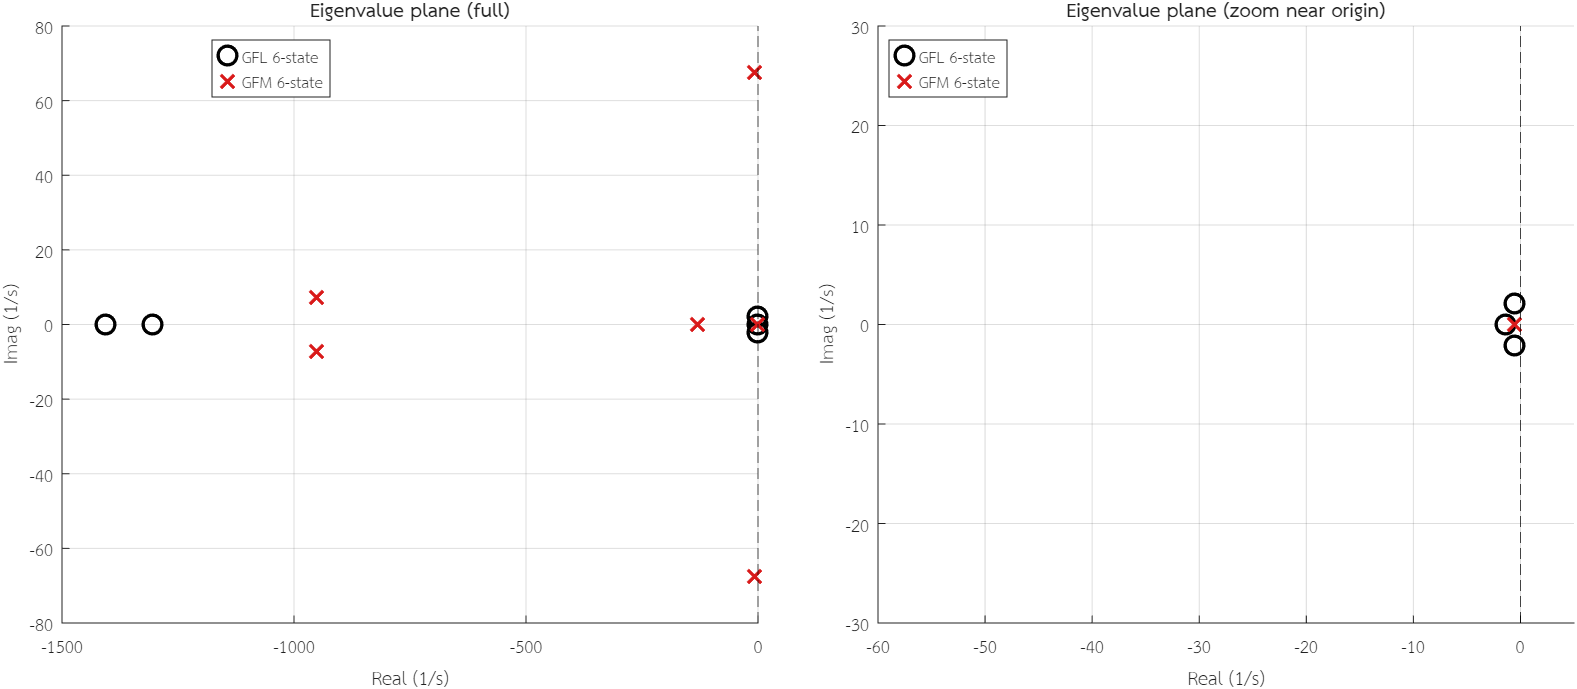
\includegraphics[width=\textwidth]{figures/ibr_gfl_gfm_th/eigenvalue_plane.png}
\caption{Eigenvalues on the complex plane (left: full, right: zoom near the origin).
Black circles = GFL 6-state, red crosses = GFM 6-state. All modes lie in the left half
plane ($\Re<0$).}
\label{fig:eigplane}
\end{figure}

\subsection{Modal frequencies (Hz)}

Figure~\ref{fig:modalfreq} shows modal frequencies in Hz. Left: oscillation frequency
$f=|\Im(\lambda)|/2\pi$ of the complex modes only (GFL PLL $\sim0.34$ Hz; GFM swing
$\sim10.8$ Hz). Right: characteristic frequency $|\lambda|/2\pi$ of every mode (log
scale), showing the spread from slow modes up to the fast current-loop modes.

\begin{figure}[H]\centering
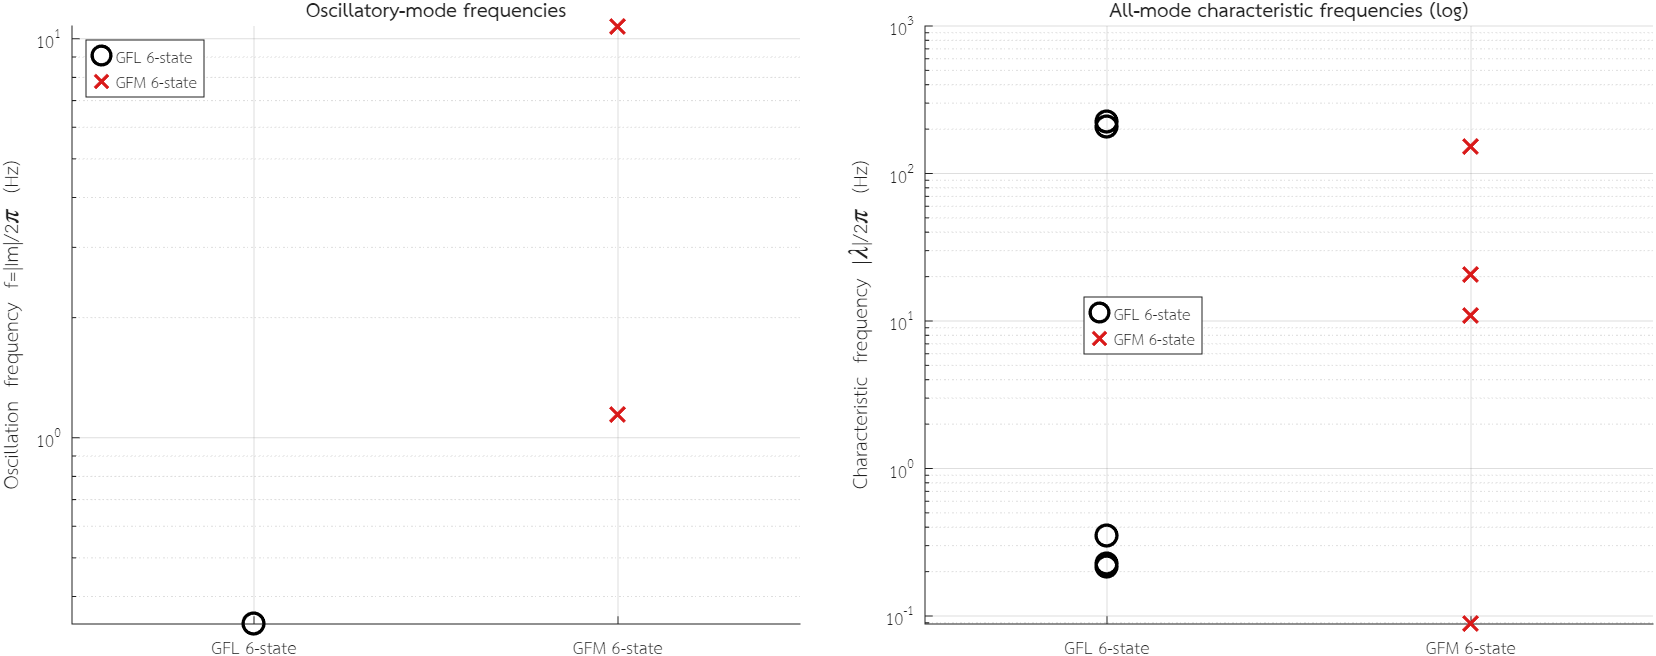
\includegraphics[width=\textwidth]{figures/ibr_gfl_gfm_th/modal_frequency.png}
\caption{Modal frequencies in Hz. Left: oscillation frequency of the complex modes;
right: characteristic frequency of all modes (log).}
\label{fig:modalfreq}
\end{figure}

\subsection{Eigenvalues under increased loading (+20\%, +40\%)}
\label{subsec:loadsweep}

To observe modal migration under \emph{increased loading} (higher $P_{ref}$, $Q$ held),
Figure~\ref{fig:eigloadsweep} shows eigenvalues at \textbf{20\%, 40\%, 60\%, 80\%, 100\%}
($P=0.2,\,0.4,\,0.6,\,0.8,\,1.0$ pu), zoomed on each model's signature oscillatory mode.
Each level re-solves the equilibrium and recomputes SSSA; all remain asymptotically
stable. The \emph{GFL PLL mode barely moves} ($0.34$ Hz throughout) while the \emph{GFM
swing mode migrates visibly} (frequency falling from $\sim10.9$ Hz at 20\% to $\sim9.5$ Hz
at 100\%).

\begin{figure}[H]\centering
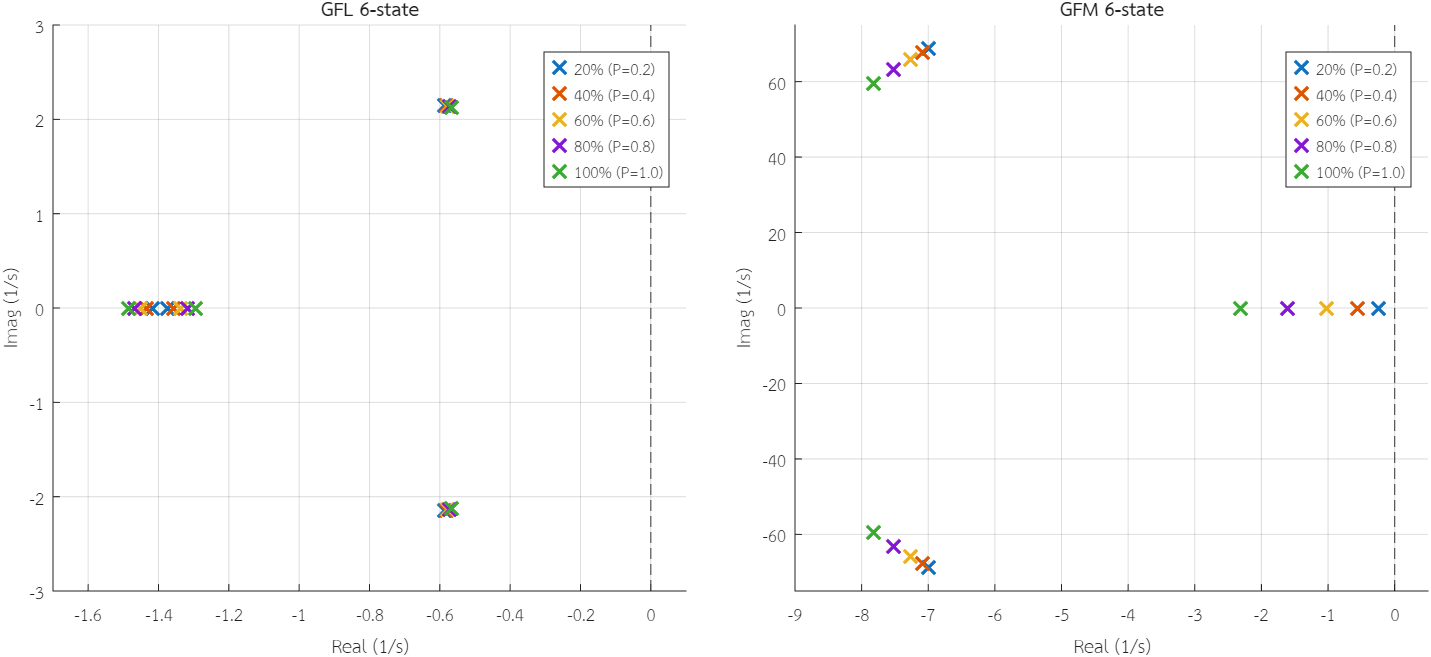
\includegraphics[width=\textwidth]{figures/ibr_gfl_gfm_th/eigenvalue_loadsweep.png}
\caption{Eigenvalues swept over 20/40/60/80/100\% load ($P=0.2$--$1.0$ pu). Left: GFL
6-state (PLL mode near the origin --- markers nearly coincide); right: GFM 6-state (swing
mode --- moves left / frequency drops with load). All points remain in the left half
plane.}
\label{fig:eigloadsweep}
\end{figure}

\subsection{Why the GFL PLL mode barely moves while the GFM swing mode migrates}
\label{subsec:whymove}

Eigenvalues come from the matrix $A$ linearised about the equilibrium. When $P_{ref}$
increases, the new operating point (load angle $\delta_0$, currents, internal voltage)
changes, so \emph{only the entries of $A$ that are nonlinear functions of the operating
point change}.

\paragraph{GFL --- PLL mode barely moves.} The GFL PLL, PQ and current loops are set by
\emph{constant gains} (eq.~\ref{eq:gfl-pll}), and the stiff SMIB terminal voltage is
nearly constant (fixed $Q$), so $A$ is almost independent of $P$; the PLL mode
($-0.58\pm j2.14$) is nearly frozen (markers overlap).

\paragraph{GFM --- swing mode moves.} Linearising the swing loop gives
\begin{equation}
s^2+\underbrace{\frac{D_v}{M}}_{\text{damping}}s+\underbrace{\frac{K_s\,\omega_b}{M}}_{\text{frequency}^2}=0,
\qquad K_s=\left.\frac{\partial P_e}{\partial\delta}\right|_0\ \propto\ \cos\delta_0,
\label{eq:swingchar}
\end{equation}
where $K_s$ is the synchronizing-power coefficient, which \emph{depends on the load
angle} $\delta_0$. As loading rises, $\delta_0$ grows, $\cos\delta_0$ falls, $K_s$
changes, and the swing mode visibly migrates (unlike the GFL, which has no load angle to
move). This is the key physical difference between \emph{tracking} (GFL) and
\emph{forming} (GFM) voltage.

\section{Comparison of $i_d,i_q,P,Q$}

Table~\ref{tab:idqpq} lists the equilibrium $i_d,i_q,P,Q$. Both models settle at the
same operating point ($P=0.40$ pu, $Q=0.10$ pu). The $i_d/i_q$ values differ because
they are expressed in different reference frames (GFL uses $\delta_{PLL}$; GFM uses the
rotor angle $\delta$), so quantitative comparison should rely on the physical $P,Q$.

\begin{table}[H]\centering\small
\caption{Equilibrium $i_d,i_q,P,Q$ of the two models ($P,Q$ on system base)}
\label{tab:idqpq}
\begin{tabular}{lcccccc}\toprule
Model & $n_x$ & $i_d$ (pu) & $i_q$ (pu) & $P$ (pu) & $Q$ (pu) & current frame\\\midrule
GFL 6-state & 6 & +0.4000 & -0.1000 & +0.4000 & +0.1000 & native\\
GFM 6-state & 6 & +0.3529 & -0.2132 & +0.4000 & +0.1000 & native\\
\bottomrule
\end{tabular}

\end{table}

The time-domain response is a fault study. Starting from the exact PF equilibrium
(static $=$ dynamic, $\|f_0\|\approx0$, so the response is \emph{flat} with no
disturbance), a shunt fault impedance $Z_f$ is applied to ground at the terminal bus over
$[t_{on},t_{clear}]$ (KCL: $I_{dev}=(V-V_{inf})/Z_{line}+V/Z_f$) and the project
implicit-trapezoidal TDS is integrated. Figure~\ref{fig:ode45gfm} (GFM) and
Figure~\ref{fig:ode45gfl} (GFL) show the response at loads 20/40/60\%: flat until the
fault, then a ring-down back to equilibrium after clearing. The GFM rings at its swing
frequency; the GFL is smoother (slow PLL mode). (Beyond $\sim70\%$ load the limiter-less
reduced GFM loses synchronism after the same fault -- a genuine transient-stability limit
of this study model.)

\begin{figure}[H]\centering
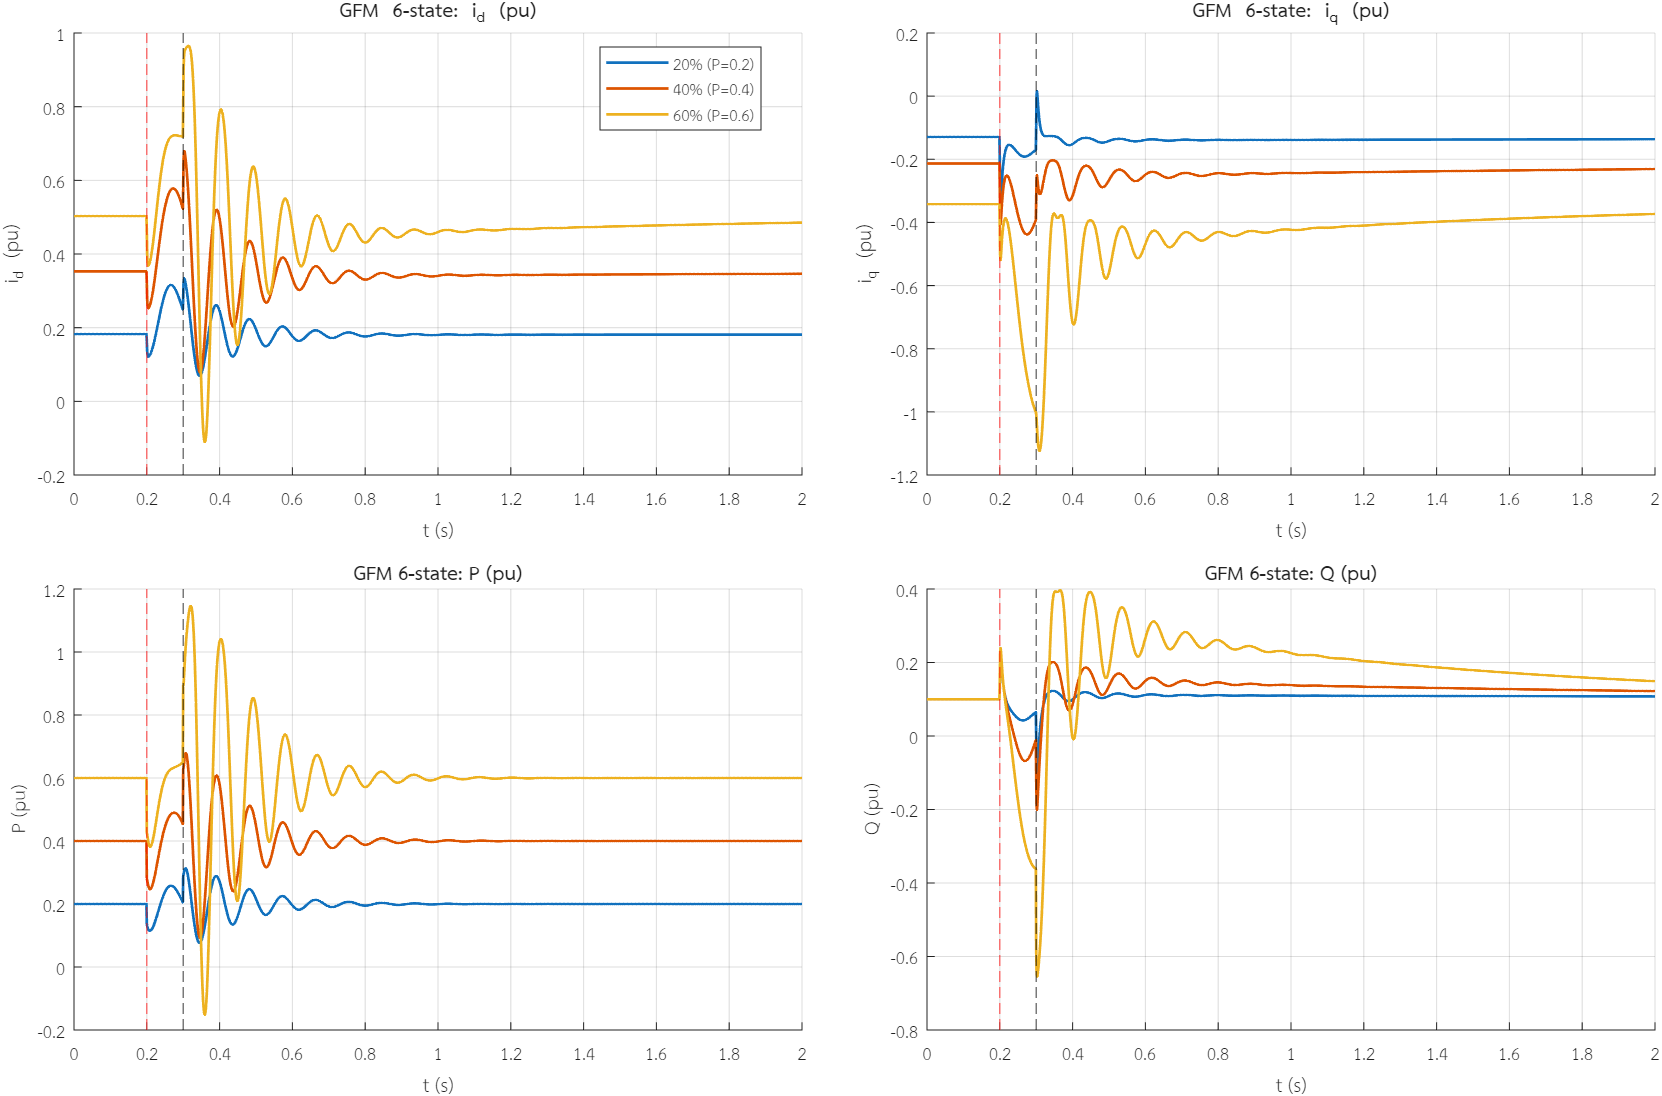
\includegraphics[width=\textwidth]{figures/ibr_gfl_gfm_th/ode45_loads_gfm.png}
\caption{GFM 6-state fault response ($Z_f=0.5j$ pu, $0.2$--$0.3$ s) at 20/40/60\% load:
flat before the fault (red = fault on, black = clear), then a swing ring-down back to
equilibrium.}
\label{fig:ode45gfm}
\end{figure}

\begin{figure}[H]\centering
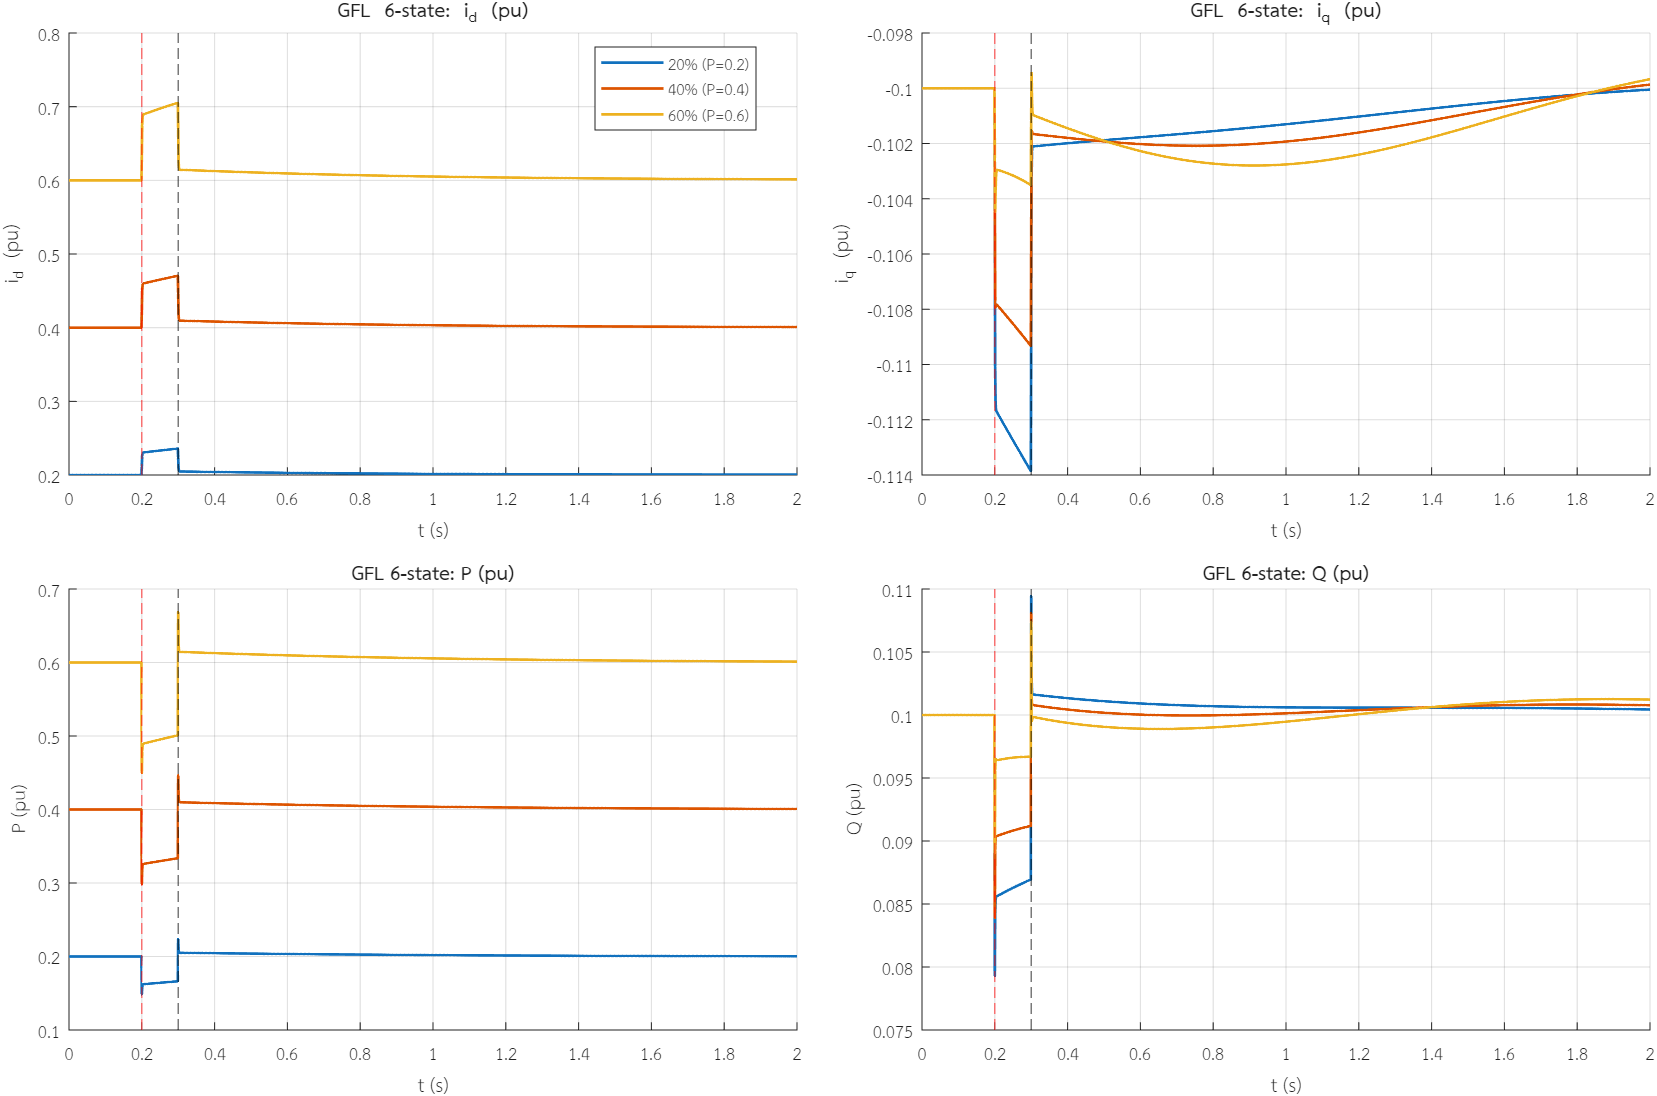
\includegraphics[width=\textwidth]{figures/ibr_gfl_gfm_th/ode45_loads_gfl.png}
\caption{GFL 6-state fault response ($Z_f=0.5j$ pu, $0.2$--$0.3$ s) at 20/40/60\% load:
flat before the fault, then a smoother recovery (slow PLL mode).}
\label{fig:ode45gfl}
\end{figure}

Finally, Figure~\ref{fig:combined} summarises \emph{everything in one figure} (15 s
simulation): frequency (dual y-axis) plus $i_d,i_q,P,Q$ for GFL (orange dashed) vs GFM
(blue solid) after the same grid step. The GFM responds fast with a wide swing (inertia,
voltage forming) while the GFL is slow and small (tracking); $P$ returns to $P_{ref}=0.4$
and the GFM $Q$ rises to support voltage after the step.

\begin{figure}[H]\centering
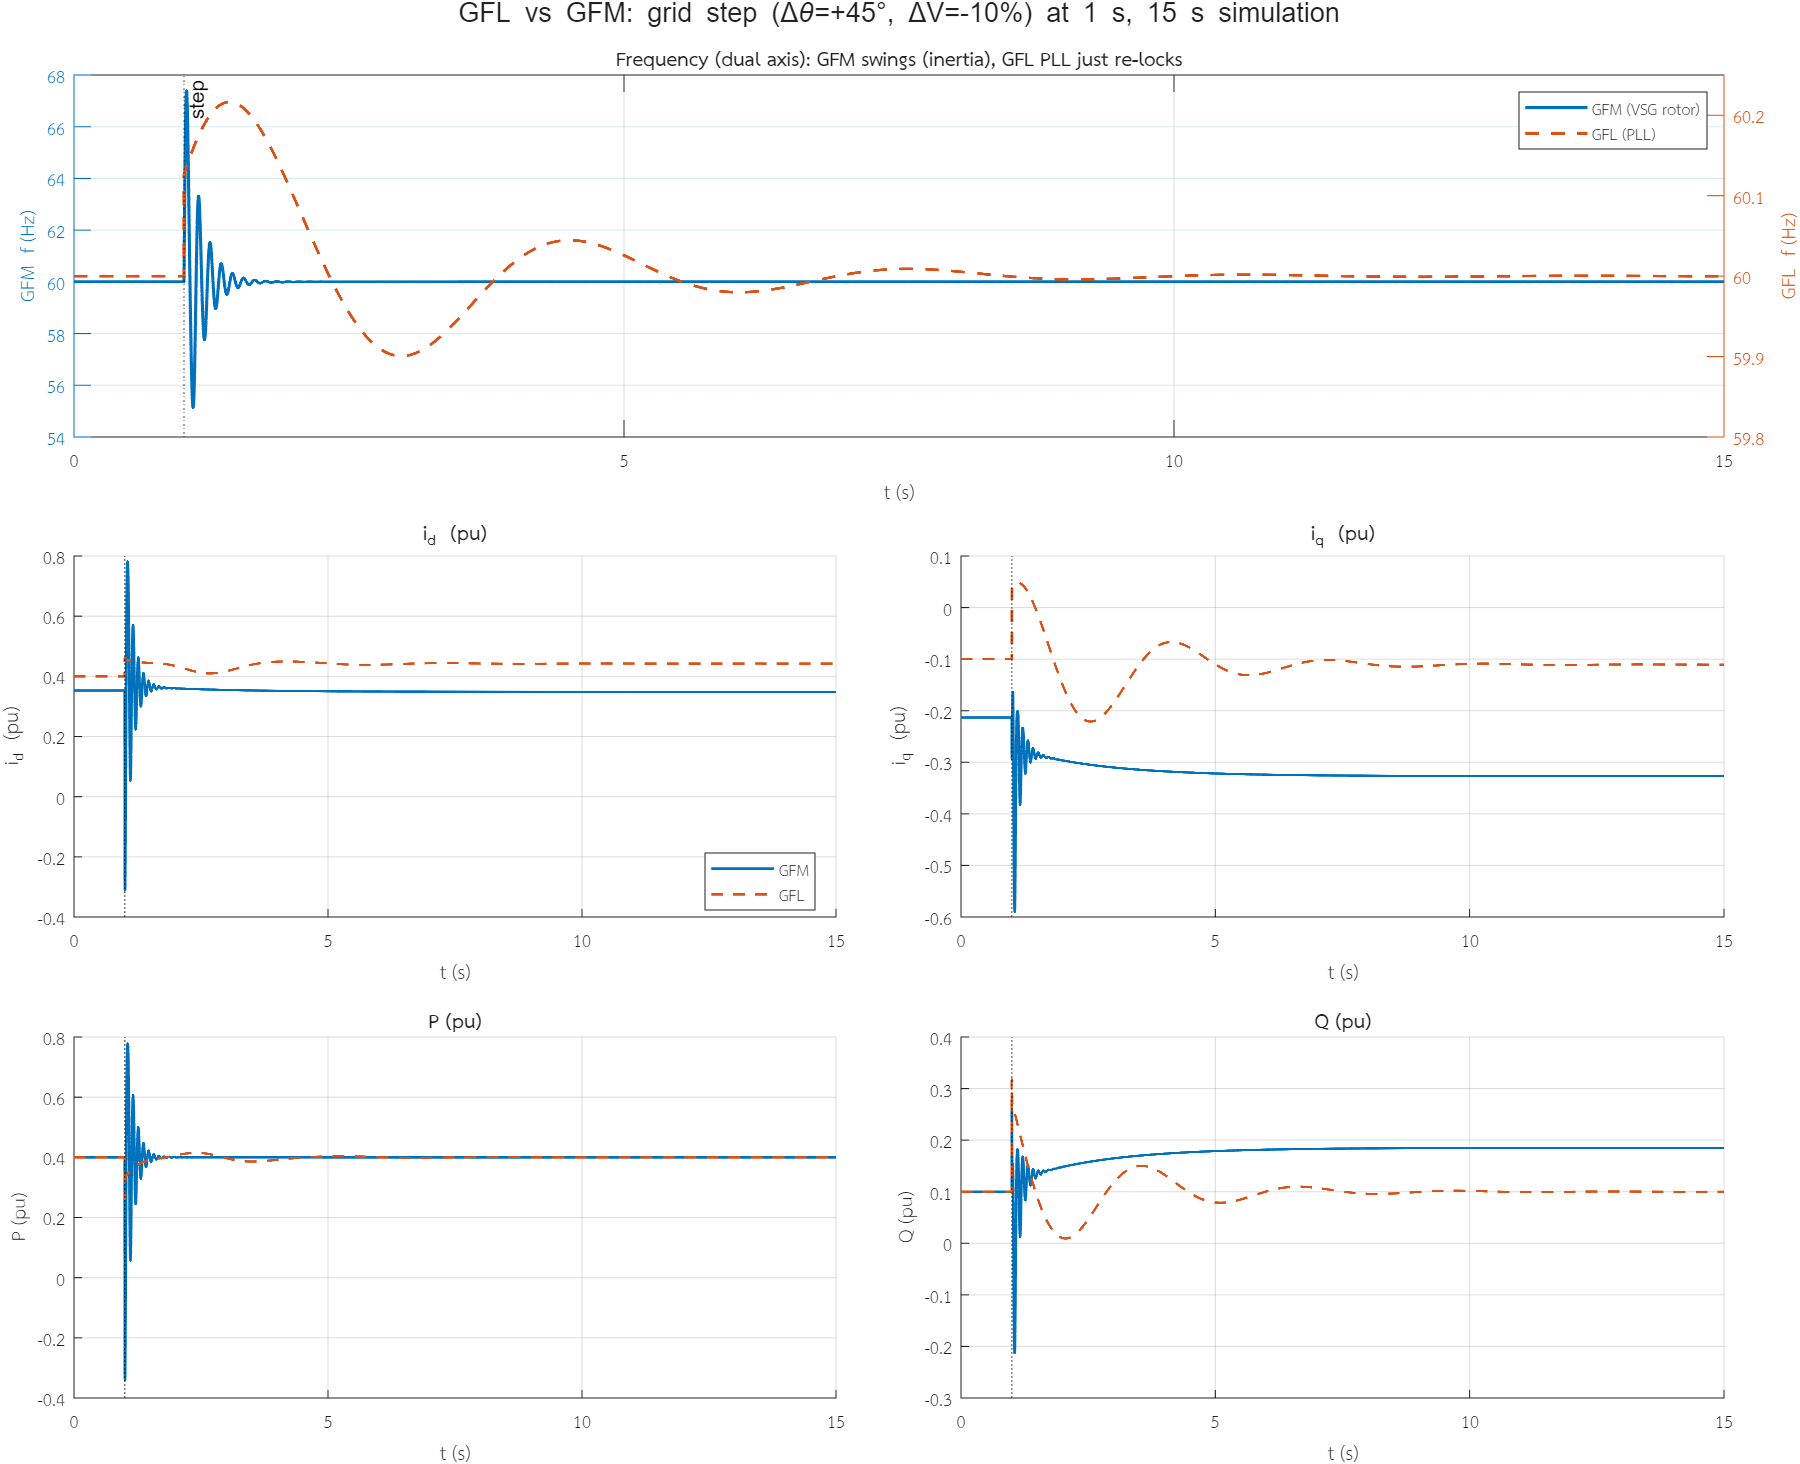
\includegraphics[width=\textwidth]{figures/ibr_gfl_gfm_th/combined_step.png}
\caption{One-figure summary: frequency (dual axis) plus $i_d,i_q,P,Q$ for GFL vs GFM after
a grid step ($\Delta\theta=+45^\circ$, $\Delta V=-10\%$) at 1 s, 15 s simulation (GFM blue
solid, GFL orange dashed).}
\label{fig:combined}
\end{figure}

\section{Conclusion}

This report presents two reduced 6-state IBR models (GFL and GFM), each organised into
three blocks of two states following the EECON49 study. Both pass the equilibrium check
(machine-precision residual) and SSSA: they are \emph{stable in every mode} and exhibit
the theoretically expected \emph{oscillatory (complex) mode} --- a PLL mode
($\sim0.34$ Hz) for the GFL and a swing mode ($\sim10.8$ Hz) for the GFM. Under
increased loading the GFL PLL mode barely moves (constant gains) whereas the GFM swing
mode migrates with the synchronizing coefficient $K_s\propto\cos\delta_0$, reflecting the
physical difference between grid-tracking and grid-forming control.

\begin{thebibliography}{9}
\bibitem{yazdani2010} A.~Yazdani and R.~Iravani, \emph{Voltage-Sourced Converters
in Power Systems: Modeling, Control, and Applications}. Hoboken, NJ: Wiley/IEEE
Press, 2010.
\bibitem{teodorescu2011} R.~Teodorescu, M.~Liserre, and P.~Rodr\'iguez,
\emph{Grid Converters for Photovoltaic and Wind Power Systems}. Chichester, UK:
Wiley/IEEE Press, 2011.
\bibitem{bacha2014} S.~Bacha, I.~Munteanu, and A.~I.~Bratcu, \emph{Power
Electronic Converters Modeling and Control}. London: Springer, 2014.
\bibitem{sakimoto2015} K.~Sakimoto, Y.~Miura, and T.~Ise, ``Virtual Synchronous
Generator without Phase Locked Loop based on Current Controlled Inverter and its
Parameter Design,'' \emph{IEEJ Trans.\ Power and Energy}, vol.~135, no.~7,
pp.~462--470, 2015.
\bibitem{pogaku2007} N.~Pogaku, M.~Prodanovi\'c, and T.~C.~Green, ``Modeling,
Analysis and Testing of Autonomous Operation of an Inverter-Based Microgrid,''
\emph{IEEE Trans.\ Power Electronics}, vol.~22, no.~2, pp.~613--625, 2007.
\bibitem{eecon49} P.~Jueajan, P.~Phadungdaen, S.~Jaingeawkham, T.~Surinkaew, and
I.~Ngamroo, ``A Bayesian Optimization-Based GFL/GFM Mode Switching Strategy for
Dynamic Stability Enhancement in Low-Inertia Power Systems,'' EECON49 (submitted),
KMITL, 2026.
\end{thebibliography}

\end{document}
